% Be sure to include the Heading Appendix A: before you type the name of the Appendix.

% Appendices should appear at the very end of your thesis. Make sure to label each Appendix with a letter starting with "A". Any tables and/or figures located in the appendix should be labeled accordingly. For example, below is figure A.1 because it is the first figure that appears in Appendix A.

\chapter{Appendix A: Flow Chart of the GS-based automated detection algorithm}\label{ch:gs-flowchart}

%If you add another appendix, copy and paste this line, but update it to B instead of A.
\renewcommand{\thechapter}{A}


\begin{figure}
    \centering
    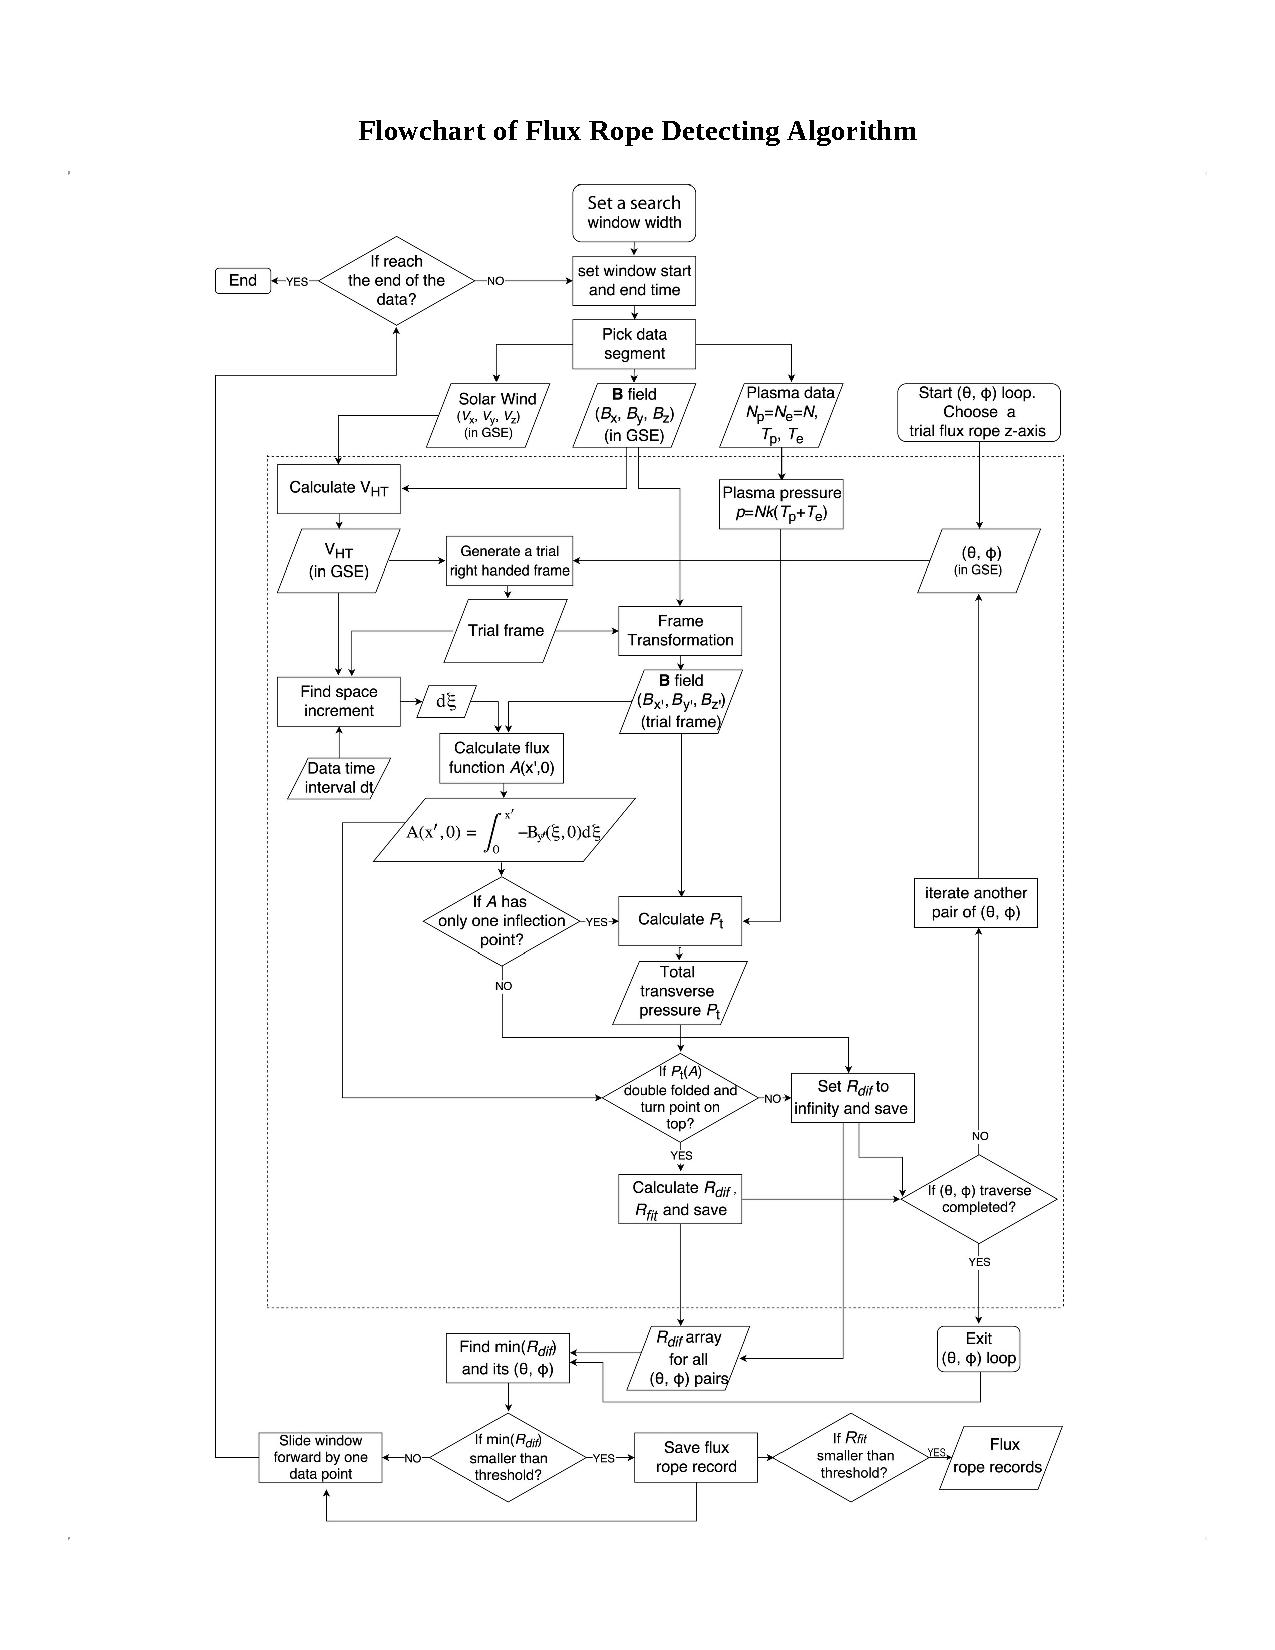
\includegraphics[width=\textwidth]{Figures/Flowchart of Flux Rope Detecting Algorithm.pdf}
    \caption[Flowchart of GS-reconstruction based automated detection algorithm]{Flowchart schematic of the automated detection algorithm of small-scale magnetic flux ropes, as implemented by \cite{Hu:2018} and \cite{Zheng:2018}.}
    \label{fig:flowchart}
\end{figure}